\documentclass[a4paper]{article}
\usepackage{geometry}
\usepackage{graphicx}
\usepackage{natbib}
\usepackage{amsmath}
\usepackage{amssymb}
\usepackage{amsthm}
\usepackage{paralist}
\usepackage{epstopdf}
\usepackage{tabularx}
\usepackage{longtable}
\usepackage{multirow}
\usepackage{multicol}
\usepackage[hidelinks]{hyperref}
\usepackage{fancyvrb}
\usepackage{algorithm}
\usepackage{algorithmic}
\usepackage{float}
\usepackage{paralist}
\usepackage[svgname]{xcolor}
\usepackage{enumerate}
\usepackage{array}
\usepackage{times}
\usepackage{url}
\usepackage{fancyhdr}
\usepackage{comment}
\usepackage{environ}
\usepackage{times}
\usepackage{textcomp}
\usepackage{caption}
\usepackage{bbm}
\usepackage{enumitem}
\usepackage{mathtools}
\usepackage{color,soul}


\urlstyle{rm}

\setlength\parindent{0pt} % Removes all indentation from paragraphs
\theoremstyle{definition}
\newtheorem{definition}{Definition}[]
\newtheorem{conjecture}{Conjecture}[]
\newtheorem{example}{Example}[]
\newtheorem{theorem}{Theorem}[]
\newtheorem{lemma}{Lemma}
\newtheorem{proposition}{Proposition}
\newtheorem{corollary}{Corollary}

\floatname{algorithm}{Procedure}
\renewcommand{\algorithmicrequire}{\textbf{Input:}}
\renewcommand{\algorithmicensure}{\textbf{Output:}}
\newcommand{\abs}[1]{\lvert#1\rvert}
\newcommand{\norm}[1]{\lVert#1\rVert}
\newcommand{\RR}{\mathbb{R}}
\newcommand{\CC}{\mathbb{C}}
\newcommand{\Nat}{\mathbb{N}}
\newcommand{\br}[1]{\{#1\}}
\DeclareMathOperator*{\argmin}{arg\,min}
\DeclareMathOperator*{\argmax}{arg\,max}
\renewcommand{\qedsymbol}{$\blacksquare$}

\definecolor{dkgreen}{rgb}{0,0.6,0}
\definecolor{gray}{rgb}{0.5,0.5,0.5}
\definecolor{mauve}{rgb}{0.58,0,0.82}

\newcommand{\Var}{\mathrm{Var}}
\newcommand{\Cov}{\mathrm{Cov}}

\newcommand{\vc}[1]{\boldsymbol{#1}}
\newcommand{\xv}{\vc{x}}
\newcommand{\Sigmav}{\vc{\Sigma}}
\newcommand{\alphav}{\vc{\alpha}}
\newcommand{\muv}{\vc{\mu}}

\newcommand{\red}[1]{\textcolor{red}{#1}}

\def\x{\mathbf x}
\def\y{\mathbf y}
\def\w{\mathbf w}
\def\v{\mathbf v}
\def\E{\mathbb E}
\def\V{\mathbb V}
\def\ind{\mathbbm 1}

% TO SHOW SOLUTIONS, include following (else comment out):
\newenvironment{soln}{
    \leavevmode\color{blue}\ignorespaces
}{}


\hypersetup{
%    colorlinks,
    linkcolor={red!50!black},
    citecolor={blue!50!black},
    urlcolor={blue!80!black}
}

\geometry{
  top=1in,            % <-- you want to adjust this
  inner=1in,
  outer=1in,
  bottom=1in,
  headheight=3em,       % <-- and this
  headsep=2em,          % <-- and this
  footskip=3em,
}


\pagestyle{fancyplain}
\lhead{\fancyplain{}{Homework 4}}
\rhead{\fancyplain{}{CS 760 Machine Learning}}
\cfoot{\thepage}

\title{\textsc{Homework 4}} % Title

%%% NOTE:  Replace 'NAME HERE' etc., and delete any "\red{}" wrappers (so it won't show up as red)

\author{
\red{$>>$Anudeep Kumar$<<$} \\
\red{$>>$9084607069$<<$}\\
} 

\date{}

\begin{document}

\maketitle 


\textbf{Instructions:} Use this latex file as a template to develop your homework. Submit your homework on time as a single pdf file to Canvas. Late submissions may not be accepted. Please wrap your code and upload it to a public GitHub repo, then attach the link below the instructions so that we can access it. You can choose any programming language (i.e. python, R, or MATLAB). Please check Piazza for updates about the homework.
Please find the link below:
\href{https://github.com/anudeepk17/HW4}{\textcolor{blue}{GiHub Link Homework 4}}

\section{Best Prediction}
\subsection{Under 0-1 Loss (10 pts)}
Suppose the world generates a single observation $x \sim \mbox{multinomial}(\theta)$, where the parameter vector $\theta=(\theta_1, \ldots, \theta_k)$ with $\theta_i\ge 0$ and $\sum_{i=1}^k \theta_i=1$.  Note $x \in \{1, \ldots, k\}$.
You know $\theta$ and want to predict $x$. 
Call your prediction $\hat x$.  What is your expected 0-1 loss: 
$$\E[\ind_{\hat x \neq x}]$$
using the following two prediction strategies respectively?  Prove your answer.
\begin{enumerate}
    \item Strategy 1: $\hat x \in \argmax_x \theta_x$, the outcome with the highest probability.
    \item Strategy 2: You mimic the world by generating a prediction $\hat x \sim \mbox{multinomial}(\theta)$.  (Hint: your randomness and the world's randomness are independent)
\end{enumerate}
\begin{soln}
    We know that $$\E[\ind_{\hat x \neq x}]=P[\hat x \neq x]$$
    This can be further expanded as 
    $$P[\hat x \neq x]=1-P[\hat x = x]$$
1. For $\hat x \in \argmax_x \theta_x$ the above formula becomes 
$$ =1-P[\hat x = \argmax_x \theta_x]$$
$$ =1- \theta_{max}$$
Where $\theta_{max} $ is the maximum $\theta$ among the probabilities
2. For $\hat x \sim \mbox{multinomial}(\theta)$
$$ = 1-P[\hat x \sim \mbox{multinomial}(\theta)]$$
Since it is given they are independent so breaking using bayes.
$$ = 1-\{p(x=1)P[\hat x =1 | x =1]+...+p(x=k)P[\hat x=k | x=k]\}$$
We know from multinomial distribution for $x$ and $\hat x $ the probabilities are $\theta_i$ so they get multiplied. 
$$\implies 1-[\theta_1^2 + \theta_2^2 +...]$$
$$\implies 1-\sum_{i=1}^k \theta_i^2$$
\end{soln}

\subsection{Under Different Misclassification Losses (6 pts)}
Like in the previous question, the world generates a single observation $x \sim \mbox{multinomial}(\theta)$. Let $c_{ij} \ge 0$ denote the loss you incur, if $x=i$ but you predict $\hat x=j$, for $i,j \in \{1, \ldots, k\}$.
$c_{ii}=0$ for all $i$. This is a way to generalize different costs of false positives vs false negatives from binary classification to multi-class classification. You want to minimize your expected loss:
$$\E[c_{x \hat x}].$$
Derive your optimal prediction $\hat x$.
\begin{soln}
    Since both $x$ and $\hat x$ are independent the cost of loss can be written as follows:
    $$
    C = \sum_{i=1}^k\sum_{j=1}^k c_{ij}\theta_i p(\hat x=j)
    $$
    Where $\theta_i$ is the prior probability of observation being ith class and the $p(\hat x=j)$ being predicting the jth class
    For $i=j \implies c_{ij}=0$
    $$
    C=\sum_{j=1}^k p(\hat x=j)\sum_{i=1}^k c_{ij}\theta_i
    $$
    Now lets assume that probability of predicting class $j$ depends on some parameter  $w$ such that
    \begin{equation}
p(\hat x ) = 
    \begin{cases}
        1 & \text{if } \hat x =w\\
        0 & \text{otherwise}
    \end{cases}
\end{equation}
So to minimize Cost we can write 
$$
argmin C = argmin _{\hat x} (\sum_{j=1}^k p(\hat x = j)\sum_{i=1 i\neq j}^k c_{ij} \theta_i)
$$
$$
argmin C = argmin _{w }(p(\hat x = w)\sum_{i=1 i\neq w}^k c_{iw}\theta_i)
$$
$$
\hat x = argmin _w(\sum_{i=1 i\neq w}^k c_{iw} \theta_i)
$$
\end{soln}
\section{Language Identification with Naive Bayes (8 pts each)}
Implement a character-based Naive Bayes classifier that classifies a document as English, Spanish, or Japanese - all written with 26 lower-case characters and space.

The dataset is languageID.tgz, unpack it. This dataset consists of 60 documents in English, Spanish, and Japanese. The correct class label is the first character of the filename: $y \in \{e, j, s\}$. (Note: here each file is a document in the corresponding language, and it is regarded as one data.)

We will be using a character-based multinomial Naïve Bayes model. You need to view each document as a bag of characters, including space. We have made sure that there are only 27 different types of printable characters (a to z, and space) -- there may be additional control characters such as new-line, please ignore those. Your vocabulary will be these 27 character types. (Note: not word types!)

In the following questions, you may use the additive smoothing technique to smooth categorical data, in case the estimated probability is zero. Given $N$ data samples $\{\vc{x}^{(i)}, y^{(i)}\}_{i = 1}^{N}$, where $\vc{x}^{(i)} = [x_1^{(i)}, \dots, x_j^{(i)}, \dots, x_{M_i}^{(i)}]$ is a bag of characters, $M_i$ is the total number of characters in $\vc{x}^{(i)}$, $x_{j}^{(i)} \in S, y^{(i)} \in L$ and we have $|S| = K_S, |L| = K_L$. Here $S$ is the set of all character types, and $L$ is the set of all classes of data labels. Then by the additive smoothing with parameter $\alpha$, we can estimate the conditional probability as 
$$
P_{\alpha}(a_s \mid y = c_k) = \frac{(\sum_{i = 1}^{N}\sum_{j = 1}^{M_i}\ind [x_{j}^{(i)} = a_s, y^{(i)} = c_k]) + \alpha}{(\sum_{b_s \in S}\sum_{i = 1}^{N}\sum_{j = 1}^{M_i}\ind [x_{j}^{(i)} = b_s, y^{(i)} = c_k]) + K_S \alpha},
$$
where $a_s \in S, c_k \in L$. Similarly, we can estimate the prior probability
$$
P_{\alpha}(Y = c_k) = \frac{(\sum_{i = 1}^{N}\ind [y^{(i)} = c_k]) + \alpha}{N + K_L \alpha},
$$
where $c_k \in L$ and $N$ is the number of training samples.
\begin{enumerate}
\item
Use files 0.txt to 9.txt in each language as the training data.
Estimate the prior probabilities 
$\hat p(y=e)$,
$\hat p(y=j)$,
$\hat p(y=s)$
using additive smoothing with parameter $\frac{1}{2}$. 
Give the formula for additive smoothing with parameter $\frac{1}{2}$ in this case. 
Print the prior probabilities.
\\
\begin{soln}
As per the formula for additive smoothing with parameter $\alpha=\frac{1}{2}$, $K_L=|L|=3$ and $N=30$ is:
    $$
    \hat{p}(y = c_k) = \frac{(\sum_{i = 1}^{30}\ind [y^{(i)} = c_k]) + 1/2}{30 + 3/2}
    $$  
For each class we 10 samples.
    \begin{align*}
        \hat{p}(y = e) = \frac{10 + 1/2}{30 + 3/2} = \frac{1}{3} \\
        \hat{p}(y = s) = \frac{10 + 1/2}{30 + 3/2} = \frac{1}{3} \\
        \hat{p}(y = j) = \frac{10 + 1/2}{30 + 3/2} = \frac{1}{3} \\
    \end{align*}
\end{soln}
\item
Using the same training data, estimate the class conditional probability (multinomial parameter) for English
$$\theta_{i,e} := \hat p(c_i \mid y=e)$$ 
where $c_i$ is the $i$-th character. That is, $c_1 = a, \ldots, c_{26} = z, c_{27} = space$.
Again, use additive smoothing with parameter $\frac{1}{2}$.
Give the formula for additive smoothing with parameter $\frac{1}{2}$ in this case. 
Print $\theta_e$ which is a vector with 27 elements.
\begin{soln}
$$
    \theta_{i,e} = \hat p(c_i \mid y=e) = \frac{(\sum_{j\in N}\sum_{k = 1}^{M_i}\ind [x_{k}^{(j)} = c_i]) + 1/2}{(\sum_{b_s \in S}\sum_{j\in N}\sum_{k = 1}^{M_i}\ind [x_{k}^{(j)} = b_s]) + 27/2}\\
    $$
    For the parameters $\alpha=\frac{1}{2}$,  $K_S=|S|=27$ 
    $$\theta_e =   \begin{bmatrix}
                            0.06017 \\
                            0.01113 \\
                            0.02151 \\
                            0.02197 \\
                            0.10537 \\
                            0.01893 \\
                            0.01748 \\
                            0.04722 \\
                            0.05541 \\
                            0.00142 \\
                            0.00373 \\
                            0.02898 \\
                            0.02052 \\
                            0.05792 \\
                            0.06446 \\
                            0.01675 \\
                            0.00056 \\
                            0.05382 \\
                            0.06618 \\
                            0.08013 \\
                            0.02666 \\
                            0.00928 \\
                            0.0155 \\
                            0.00116 \\
                            0.01384 \\
                            0.00063 \\
                            0.17925 \\
                        \end{bmatrix}$$
\end{soln}

\item
Print $\theta_j, \theta_s$, the class conditional probabilities for Japanese and Spanish.
\begin{soln}
\[
        \left
    
        \theta_{j} =\begin{bmatrix}
                        0.13177 \\
                        0.01087 \\
                        0.00549 \\
                        0.01723 \\
                        0.0602 \\
                        0.00388 \\
                        0.01401 \\
                        0.03176 \\
                        0.09703 \\
                        0.00234 \\
                        0.05741 \\
                        0.00143 \\
                        0.0398 \\
                        0.05671 \\
                        0.09116 \\
                        0.00087 \\
                        0.0001 \\
                        0.0428 \\
                        0.04217 \\
                        0.05699 \\
                        0.07062 \\
                        0.00024 \\
                        0.01974 \\
                        3e-05 \\
                        0.01415 \\
                        0.00772 \\
                        0.12345 \\
                    \end{bmatrix}
    %
    \right
        \theta_{s}=\begin{bmatrix}
                        0.10456 \\
                        0.00823 \\
                        0.03753 \\
                        0.03975 \\
                        0.11381 \\
                        0.0086 \\
                        0.00718 \\
                        0.00453 \\
                        0.04986 \\
                        0.00663 \\
                        0.00028 \\
                        0.05294 \\
                        0.02581 \\
                        0.05418 \\
                        0.07249 \\
                        0.02427 \\
                        0.00768 \\
                        0.0593 \\
                        0.06577 \\
                        0.03561 \\
                        0.0337 \\
                        0.00589 \\
                        9e-05 \\
                        0.0025 \\
                        0.00786 \\
                        0.00268 \\
                        0.16826 \\
        \end{bmatrix}
        \]
   
\end{soln}

\item
Treat e10.txt as a test document $x$.
Represent $x$ as a bag-of-words count vector (Hint: the vocabulary has size 27).
Print the bag-of-words vector $x$.

    \begin{soln}
        $x = [164\;32\;53\;57\;311\;55\;51\;140\;140\;3\;6\;85\;64\;139\;182\;53\;3\;141\;186\;225\;65\;31\;47\;4\;38\;2\;498]$
\end{soln}


\item
For the $x$ of e10.txt, compute $\hat p(x \mid y)$ for $y=e, j, s$ under the multinomial model assumption, respectively.
Use the formula
$$\hat p(x \mid y) = \prod_{i=1}^d (\theta_{i, y})^{x_i}$$
where $x=(x_1, \ldots, x_d)$.
Show the three values: $\hat p(x \mid y=e), \hat p(x \mid y=j), \hat p(x \mid y=s)$.

Hint: you may notice that we omitted the multinomial coefficient.  This is ok for classification because it is a constant w.r.t. $y$. Also, Store all probabilities here and below in $\log()$ internally to avoid underflow. This also means you need to do arithmetic in log space. \\
\begin{soln}
    There was an underflow issue , and because of that, the problem was solved in the log space using the following formula. We know that log is an increasing function it follows the same comparison rules as the original probabilities.
    $$
        \hat p(x \mid y) = \prod_{i=1}^d (\theta_{i, y})^{x_i}
        $$
        $$
        \log(\hat p(x \mid y)) = \sum_{i=1}^d\log((\theta_{i, y})^{x_i})
        $$
        $$
        \log(\hat p(x \mid y)) = \sum_{i=1}^d x_i\log(\theta_{i, y})
        $$
        $$
        \hat p(x \mid y) = e^{\sum_{i=1}^d x_i\log(\theta_{i, y})}
    $$
    
    Thus the condition probabilities are:
    $$
        \hat p(x \mid y=e) = e^{-7841.8654}
        $$
        $$
        \hat p(x \mid y=s) = e^{-8467.2820}
        $$
        $$
        \hat p(x \mid y=j) = e^{-8771.4331}
    $$
\end{soln}

\item
For the $x$ of e10.txt, use the Bayes rule and your estimated prior and likelihood, compute the posterior $\hat p(y \mid x)$.
Show the three values: $\hat p(y=e \mid x), \hat p(y=j \mid x), \hat p(y=s \mid x)$.
Show the predicted class label of $x$.
\begin{soln}
    \begin{align*}
        \hat p(y \mid x) &= \frac{\hat p(x \mid y) \hat p(y)}{\hat p(x)} \\
        \hat p(y=e \mid x) &= \frac{\hat p(x \mid y=e) \hat p(y=e)}{\hat p(x)} = \frac{1}{3}\cdot\frac{e^{-7841.8654}}{\hat p(x)}\\
        \hat p(y=s \mid x) &= \frac{\hat p(x \mid y=s) \hat p(y=s)}{\hat p(x)} = \frac{1}{3}\cdot\frac{e^{-8467.2820}}{\hat p(x)}\\
        \hat p(y=j \mid x) &= \frac{\hat p(x \mid y=j) \hat p(y=j)}{\hat p(x)} = \frac{1}{3}\cdot\frac{e^{-8771.4331}}{\hat p(x)}
    \end{align*}
    We know that $\hat p(x)$ is positive, therefore the predicted class is: 
    $$
    \argmax_{c_i\in\{e,s,j\}} \hat p(y=c_i \mid x) = \mathbf{e}
    $$
    Thus the predicted class for \texttt{e10.txt} is \textbf{English}
\end{soln}
\item
Evaluate the performance of your classifier on the test set (files 10.txt to 19.txt in three languages).
Present the performance using a confusion matrix. A confusion matrix summarizes the types of errors your classifier makes, as shown in the table below.   The columns are the true language a document is in, and the rows are the classified outcome of that document.  The cells are the number of test documents in that situation.  For example, the cell with row = English and column = Spanish contains the number of test documents that are really Spanish but misclassified as English by your classifier.

\begin{soln}
    \begin{center}
        \begin{tabular}{c|ccc}
            & English & Spanish & Japanese \\
            \hline
            English&10&0&0\\
            Spanish&0&10&0\\
            Japanese&0&0&10
        \end{tabular}
    \end{center}
\end{soln}

\item Take a test document.   Arbitrarily shuffle the order of its characters so that the words (and spaces) are scrambled beyond human recognition.  How does this shuffling affect your Naive Bayes classifier's prediction on this document?  Explain the key mathematical step in the Naive Bayes model that justifies your answer.\\
\begin{soln}
    Using \texttt{j6.txt}, we get the exact prediction of \textbf{Japanese}.The Naive Bayes technique used here only \hl{counts the number of characters} in the sentence \hl{without caring about their relative position}. Thus even after shuffling them, their representation in the model is precisely the same as before, and we get the same output.

    The critical mathematical step which achieves this is the \textbf{calculation of conditional probability} where the \hl{probability} of each feature \hl{is calculated solely based on the class}. There is \hl{no dependence between the features themselves} thus the relative placement of characters is not important to the model anymore.
\end{soln}

\end{enumerate}

\section{Simple Feed-Forward Network (20pts)}
In this exercise, you will derive, implement back-propagation for a simple neural network and compare your output with some standard library’s output. Consider the following 3-layer neural network.

\[
\hat{y} = f(x) = g(W_3\sigma(W_2\sigma(W_1x)))
\]

Suppose $x \in \mathbb{R}^d$, $W_1 \in \mathbb{R}^{d_1 \times d}$, $W_2 \in \mathbb{R}^{d_2 \times d_1}$, $W_3 \in \mathbb{R}^{k \times d_2}$ i.e. $f: \mathbb{R}^d \rightarrow \mathbb{R}^k$, Let $\sigma(z) = [\sigma(z_1), ..., \sigma(z_n)]$ for any $z \in \mathbb{R}^n$ where $\sigma(z) = \frac{1}{1 + e^{-z}}$ is the sigmoid (logistic) activation function and $g(z_i) = \frac{exp(z_i)}{\sum_{i=1}^k exp(z_i)}$ is the softmax function. Suppose the true pair is $(x, y)$ where $y \in \{0, 1\}^k$ with exactly one of the entries equal to 1, and you are working with the cross-entropy loss function given below,

\[
L(x, y) = -\sum_{i=1}^k y \text{log}(\hat{y})
\]

\begin{enumerate}
    \item Derive backpropagation updates for the above neural network. (5 pts)
    \begin{soln}
    We have two functions. To find the backpropagation update we need to first understand the derivative of each of the function. 
    Let us first understand how each nueron of the network is getting its input. If we name the $ith$ nueron of first layer as $t_i$, second as $u_i$ and third as $y_i$. and the weights are matrices as per $W_1 \in \mathbb{R}^{d_1 \times d}$, $W_2 \in \mathbb{R}^{d_2 \times d_1}$, $W_3 \in \mathbb{R}^{k \times d_2}$  Then we can write the $ith$ nueron as 
    $$
    t_i=\sigma(W1_{i1}x_1+...W1_{id}x_d)
    $$
    $$
    u_i=\sigma(W2_{i1}t_1+...W1_{id_1}t_{d_1})
    $$
    $$
    \hat y_i=\frac{\exp(W3_{i1}u_1+...W3_{id_2}u_{d_2})}{\sum_{i=1}^k \exp(W3_{i1}u_1+...W3_{id_2}u_{d_2})}
    $$
    Now to update each layers weights we find the derivative of $\hat y$ with respect to the corresponding weights
    Therefore,
    $$
    \frac{\partial{\hat y_i}}{\partial{W3_{ij}}}
    $$
    can have 2 cases, \\
    Case 1 : Finding derivative of $\hat y_i$ with respect to
    $
    W3_{ij}
    $
    $$
    \frac{\partial{\hat y_i}}{\partial{W3_{ij}}}=\frac{\exp(W3_{i1}u_1+...W3_{id_2}u_{d_2})}{\sum_{i=1}^k \exp(W3_{i1}u_1+...W3_{id_2}u_{d_2})}u_j-(\frac{\exp(W3_{i1}u_1+...W3_{id_2}u_{d_2})}{\sum_{i=1}^k \exp(W3_{i1}u_1+...W3_{id_2}u_{d_2})})^2u_j
    $$
    \\
    $$
    \implies \frac{\partial{\hat y_i}}{\partial{W3_{ij}}}=\hat y_iu_j(1-\hat y_iu_j)
    $$
    Case 2 : Finding derivative $\hat y_i$ with respect to $W3_{mj}$
    $$
    \frac{\partial{\hat y_i}}{\partial{W3_{mj}}}=0-\frac{\exp(W3_{i1}u_1+...W3_{id_2}u_{d_2})}{(\sum_{i=1}^k \exp(W3_{i1}u_1+...W3_{id_2}u_{d_2}))^2}\exp(W3_{m1}u_1+..+W3_{mj}u_j..+W3_{md_2}u_{d_2})u_j
    $$
    $$
    \frac{\partial{\hat y_i}}{\partial{W3_{mj}}}=0-\frac{\exp(W3_{i1}u_1+...W3_{id_2}u_{d_2})}{\sum_{i=1}^k \exp(W3_{i1}u_1+...W3_{id_2}u_{d_2})}\frac{\exp(W3_{m1}u_1+...W3_{md_2}u_{d_2})}{\sum_{i=1}^k \exp(W3_{i1}u_1+...W3_{id_2}u_{d_2})}u_j
    $$
    $$
    \implies \frac{\partial{\hat y_i}}{\partial{W3_{mj}}}=-\hat y_i\hat y_mu_j
    $$
    Therefore generalising the above observation for softmax we can easily conclude for a function of variable $z$ we can write the derivative of the function as 
    \begin{equation}
\frac{\partial{\hat y_i}}{\partial{z}}=
    \begin{cases}
        \hat y_i(1-\hat y_i) & \text{if } i=j\\
        -\hat y_i \hat y_j & \text{if } i\neq j
    \end{cases}
\end{equation}


    Now to compute the backpropogation GD we need to write formula of loss and differentiate with respect to each weight
$$
L(x, y) = -\sum_{i=1}^k y \text{log}(\hat{y})
$$
Where $\hat y$ is a function of say $z$
$$
\frac{\partial{L}}{\partial{z}}=\frac{\partial{\sum_{i=1}^k y_i log(\hat y_i)}}{\partial{z}}
$$
$$
\implies \sum_{i=1}^k \frac{-y_i}{\hat y_i}\frac{\partial{\hat y_i}}{\partial{z}}
$$
From the above conclusion
$$
\implies
\frac{\partial{L}}{\partial{z}}=\frac{-y_i}{\hat y_i}\hat{y_i}(1-\hat{y_i}) + \sum_{j\neq i}\frac{y_j}{\hat y_j}\hat{y_j}\hat{y_i}
$$
$$
\implies
\frac{\partial{L}}{\partial{z}}=-y_i+y_i\hat{y_i}+\sum_{j\neq i}y_j\hat{y_i}
$$
$$
\implies
\frac{\partial{L}}{\partial{z}}=-y_i+\hat{y_i}(\sum_{j\neq i}y_j+y_i)
$$
The term with $\hat{y_j}$ sums to 1

$$
\implies
\frac{\partial{L}}{\partial{z}}=\hat{y_i}-y_i
$$
Now for layers behind the first layer we continue considering the $u,t,x$ terms
We know that the derivative of sigmoid is 
$$
\frac{\partial{\sigma(z)}}{\partial{z}}=\sigma(z)(1-\sigma(z))
$$
Using the above , for 
$$
\frac{\partial{L}}{\partial{W3}}=\frac{\partial{L}}{\partial{u}}\frac{\partial{u}}{\partial{W3}}
$$
Let
$$
A1=(W_2\sigma(W_1x))
$$
$$
\implies
\frac{\partial{L}}{\partial{W_3}}=(\hat{y_i}-y_i)(\sigma(A1))\partial((W_3))/\partial(W_3)
$$
$$
\implies
\frac{\partial{L}}{\partial{W_3}}=(\hat{y_i}-y_i)\sigma(A1)
$$
Similarly
$$
A2=\sigma(W_1x)
$$
$$
L=g(W_3\sigma(W_2A2))
$$
$$
\implies
\frac{\partial{L}}{\partial{W_2}}=(\hat{y_i}-y_i)(W_3)\frac{\partial{\sigma(W_2A2)}}{\partial{W_2}}
$$
$$
\implies
\frac{\partial{L}}{\partial{W_2}}=(\hat{y_i}-y_i)(W_3)\sigma(W_2A2)(1-\sigma(W_2A2))A2
$$
Similarly

$$
L=g(W_3\sigma(W_2\sigma(W_1x))
$$
$$
\implies
\frac{\partial{L}}{\partial{W_1}}=(\hat{y_i}-y_i)(W_3)\frac{\partial{\sigma(W_2\sigma(W_1x))}}{\partial{W_1}}
$$

$$
\implies
\frac{\partial{L}}{\partial{W_1}}=(\hat{y_i}-y_i)(W_3)\sigma(W_2\sigma(W_1x))(1-\sigma(W_2\sigma(W_1x)))W2\frac{\partial{\sigma(W_1x))}}{\partial{W_1}}
$$
$$
\implies
\frac{\partial{L}}{\partial{W_1}}=(\hat{y_i}-y_i)(W_3)\sigma(W_2\sigma(W_1x))(1-\sigma(W_2\sigma(W_1x)))W2\sigma(W_1x)(1-\sigma(W_1x))x
$$
    \end{soln}
    \item Implement it in NumPy or PyTorch using basic linear algebra operations. (e.g. You are not allowed to use auto-grad, built-in optimizer, model, etc. in this step. You can use library functions for data loading, processing, etc.). Evaluate your implementation on MNIST dataset, report test errors and learning curve. (10 pts) \\
    \begin{soln}
        Case 1: $\\
        \alpha = 0.01 \\
        BatchSize = 32 \\
         $
         Epoch: 50, Test Error Percent: 6.83, Loss: 0.22
\begin{figure}[H]
            
                \centering
                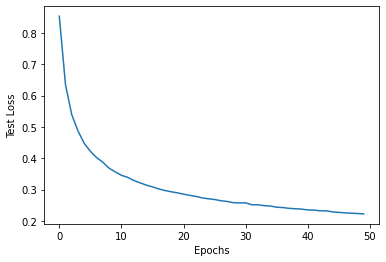
\includegraphics[scale=0.5]{Images/scratch32_0.01_random.png}
            
        \end{figure}     
         Case 2: $\\
        \alpha = 0.01 \\
        BatchSize = 64 \\
        $
        Epoch: 50, Test Error Percent: 8.02, Loss: 0.26
        \begin{figure}[H]
            
                \centering
                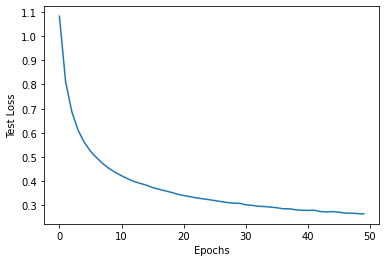
\includegraphics[scale=0.5]{Images/scratch64_0.01_random.png}
            
        \end{figure} 
        Case 3: $\\
        \alpha = 0.001 \\
        BatchSize = 32 \\
        $
        Epoch: 50, Test Error Percent: 13.55, Loss: 0.45
        \begin{figure}[H]
            
                \centering
                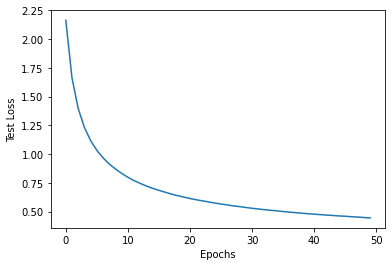
\includegraphics[scale=0.5]{Images/scratch32_0.001_random.png}
            
        \end{figure} 
    \end{soln}
    \item Implement the same network in PyTorch (or any other framework). You can use all the features of the framework e.g. auto-grad etc. Evaluate it on MNIST dataset, report test errors, and learning curve. (2 pts)
       \begin{soln}
        Case 1: $\\
        \alpha = 0.01 \\
        BatchSize = 32 \\
         $
         Epoch:  50 \\
    Running loss:  0.1504874899893999 \\

    Accuracy Percent: 57419/60000 (96\%) \\


Test Error Percent: (4 \%) \\
\begin{figure}[H]
            
                \centering
                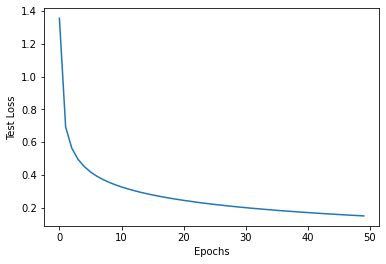
\includegraphics[scale=0.5]{Images/py32_0.01_random.png}
            
        \end{figure}     
         Case 2: $\\
        \alpha = 0.01 \\
        BatchSize = 64 \\
        $
       Epoch:  50 \\
    Running loss:  0.22683055126574883 \\

    Accuracy Percent: 55953/60000 (93\%) \\


Test Error Percent: (7\%) \\
        \begin{figure}[H]
            
                \centering
                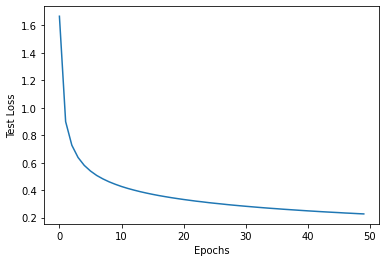
\includegraphics[scale=0.5]{Images/py64_0.01_random.png}
            
        \end{figure}     
        Case 3: $\\
        \alpha = 0.001 \\
        BatchSize = 32 \\
        $
       Epoch:  50 \\
Running loss:  0.44513462127049763 \\

Accuracy Percent: 51672/60000 (86 \%)


Test Error Percent: (14\%)

        \begin{figure}[H]
            
                \centering
                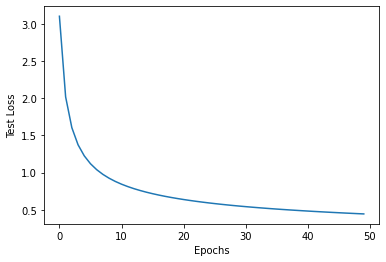
\includegraphics[scale=0.5]{Images/py32_0.001_random.png}
            
        \end{figure}     
    \end{soln}
    \item Try different weight initialization a) all weights initialized to 0, and b) initialize the weights randomly between -1 and 1. Report test error and learning curves for both. (You can use either of the implementations) (3 pts)
\end{enumerate}
\begin{soln}
     Case 1: $\\
        \alpha = 0.01 \\
        BatchSize = 32 \\
         $
         Running loss:  0.7020412162303925 \\

Accuracy Percent: 47758/60000 (80\%) \\


Test Error Percent: (20\%) \\
\begin{figure}[H]
            
                \centering
                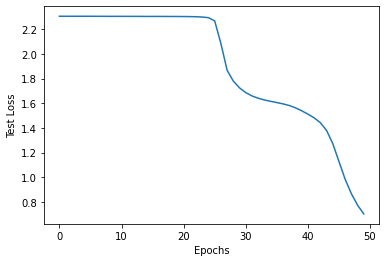
\includegraphics[scale=0.5]{Images/py32_0.01_zero.png}
            
        \end{figure}   

        Case 2: $\\
        \alpha = 0.01 \\
        BatchSize = 32 \\
         $
         Epoch:  50 \\
    Running loss:  0.1504874899893999 \\

    Accuracy Percent: 57419/60000 (96\%) \\


Test Error Percent: (4 \%) \\
\begin{figure}[H]
            
                \centering
                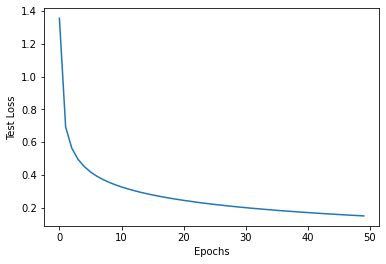
\includegraphics[scale=0.5]{Images/py32_0.01_random.png}
            
        \end{figure}      


\end{soln}
You should play with different hyperparameters like learning rate, batch size, etc. for your own learning. You only need to report results for any particular setting of hyperparameters. You should mention the values of those along with the results. Use $d_1 = 300$, $d_2 = 200$, $d_3 = 100$. For optimization use SGD (Stochastic gradient descent) without momentum, with some batch size say 32, 64, etc. MNIST can be obtained from here (https://pytorch.org/vision/ stable/datasets.html)

\bibliographystyle{apalike}
\end{document}
